% Options for packages loaded elsewhere
\PassOptionsToPackage{unicode}{hyperref}
\PassOptionsToPackage{hyphens}{url}
%
\documentclass[
]{book}
\usepackage{amsmath,amssymb}
\usepackage{iftex}
\ifPDFTeX
  \usepackage[T1]{fontenc}
  \usepackage[utf8]{inputenc}
  \usepackage{textcomp} % provide euro and other symbols
\else % if luatex or xetex
  \usepackage{unicode-math} % this also loads fontspec
  \defaultfontfeatures{Scale=MatchLowercase}
  \defaultfontfeatures[\rmfamily]{Ligatures=TeX,Scale=1}
\fi
\usepackage{lmodern}
\ifPDFTeX\else
  % xetex/luatex font selection
\fi
% Use upquote if available, for straight quotes in verbatim environments
\IfFileExists{upquote.sty}{\usepackage{upquote}}{}
\IfFileExists{microtype.sty}{% use microtype if available
  \usepackage[]{microtype}
  \UseMicrotypeSet[protrusion]{basicmath} % disable protrusion for tt fonts
}{}
\makeatletter
\@ifundefined{KOMAClassName}{% if non-KOMA class
  \IfFileExists{parskip.sty}{%
    \usepackage{parskip}
  }{% else
    \setlength{\parindent}{0pt}
    \setlength{\parskip}{6pt plus 2pt minus 1pt}}
}{% if KOMA class
  \KOMAoptions{parskip=half}}
\makeatother
\usepackage{xcolor}
\usepackage{longtable,booktabs,array}
\usepackage{calc} % for calculating minipage widths
% Correct order of tables after \paragraph or \subparagraph
\usepackage{etoolbox}
\makeatletter
\patchcmd\longtable{\par}{\if@noskipsec\mbox{}\fi\par}{}{}
\makeatother
% Allow footnotes in longtable head/foot
\IfFileExists{footnotehyper.sty}{\usepackage{footnotehyper}}{\usepackage{footnote}}
\makesavenoteenv{longtable}
\usepackage{graphicx}
\makeatletter
\def\maxwidth{\ifdim\Gin@nat@width>\linewidth\linewidth\else\Gin@nat@width\fi}
\def\maxheight{\ifdim\Gin@nat@height>\textheight\textheight\else\Gin@nat@height\fi}
\makeatother
% Scale images if necessary, so that they will not overflow the page
% margins by default, and it is still possible to overwrite the defaults
% using explicit options in \includegraphics[width, height, ...]{}
\setkeys{Gin}{width=\maxwidth,height=\maxheight,keepaspectratio}
% Set default figure placement to htbp
\makeatletter
\def\fps@figure{htbp}
\makeatother
\setlength{\emergencystretch}{3em} % prevent overfull lines
\providecommand{\tightlist}{%
  \setlength{\itemsep}{0pt}\setlength{\parskip}{0pt}}
\setcounter{secnumdepth}{5}
\usepackage{booktabs}
\ifLuaTeX
  \usepackage{selnolig}  % disable illegal ligatures
\fi
\usepackage[]{natbib}
\bibliographystyle{plainnat}
\IfFileExists{bookmark.sty}{\usepackage{bookmark}}{\usepackage{hyperref}}
\IfFileExists{xurl.sty}{\usepackage{xurl}}{} % add URL line breaks if available
\urlstyle{same}
\hypersetup{
  pdftitle={Topology},
  pdfauthor={Ashan Jayamal},
  hidelinks,
  pdfcreator={LaTeX via pandoc}}

\title{Topology}
\author{Ashan Jayamal}
\date{2024-02-13}

\usepackage{amsthm}
\newtheorem{theorem}{Theorem}[chapter]
\newtheorem{lemma}{Lemma}[chapter]
\newtheorem{corollary}{Corollary}[chapter]
\newtheorem{proposition}{Proposition}[chapter]
\newtheorem{conjecture}{Conjecture}[chapter]
\theoremstyle{definition}
\newtheorem{definition}{Definition}[chapter]
\theoremstyle{definition}
\newtheorem{example}{Example}[chapter]
\theoremstyle{definition}
\newtheorem{exercise}{Exercise}[chapter]
\theoremstyle{definition}
\newtheorem{hypothesis}{Hypothesis}[chapter]
\theoremstyle{remark}
\newtheorem*{remark}{Remark}
\newtheorem*{solution}{Solution}
\begin{document}
\maketitle

{
\setcounter{tocdepth}{1}
\tableofcontents
}
\hypertarget{topology}{%
\chapter{Topology}\label{topology}}

A topology is a geometric structure defined on a set. Basically it is given by declaring which subsets are ``open'' sets. Thus the axioms are the abstraction of the properties that open sets have.

\hypertarget{topological-spaces}{%
\section{Topological Spaces}\label{topological-spaces}}

\begin{definition}
\protect\hypertarget{def:Top}{}\label{def:Top}A topology on a set \(X\) is a collection \(\mathcal{T}\) of subsets of \(X\) such that

(T1) \(\phi\) and \(X\) are in \(\mathcal{T}\);

(T2) Any union of subsets in \(\mathcal{T}\) is in \(\mathcal{T}\);

(T3) The finite intersection of subsets in \(\mathcal{T}\) is in \(\mathcal{T}\).
\end{definition}

A set \(X\) with a topology \(\mathcal{T}\) is called a topological space. Denoted by \((X,\mathcal{T})\). An element of \(\mathcal{T}\) is called an open set.

\begin{example}
\protect\hypertarget{exm:unnamed-chunk-1}{}\label{exm:unnamed-chunk-1}Let \(X\) be a three-element set, \(X = \{a, b, c\}\) and \(\tau=\{X, \emptyset,\{a, b\}, \{b\}, \{b, c\}\}\). We can check T1,T2 and T3 conditions.
\end{example}

\begin{example}
\protect\hypertarget{exm:unnamed-chunk-2}{}\label{exm:unnamed-chunk-2}Let \(X\) be a three-element set, \(X = \{a, b, c\}\) as pervoius. There are many possible topologies on \(X\), some of which are indicated schematically in figure \ref{fig:gi}. Furthur, we can see that even a three-element set has many different topologies.
\end{example}

\begin{figure}
\centering
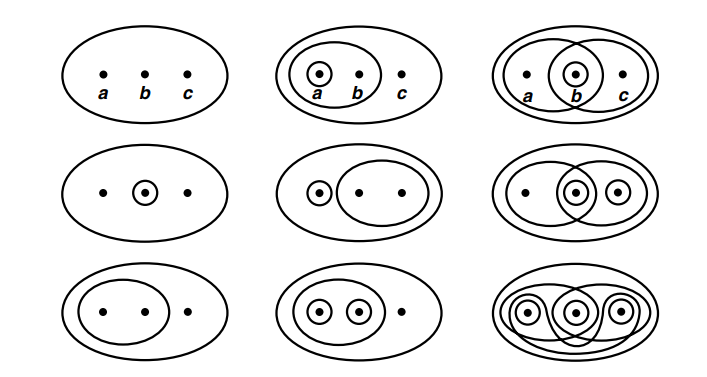
\includegraphics{figure 01.png}
\caption{\label{fig:gi}\(~\)}
\end{figure}

\begin{remark}
Not every collection of subsets of \(X\) is a topology on \(X\). Observe that Neither of the collections indicated in figure \ref{fig:fig2} is a topology.

First let's consider the left hand coner of figure \ref{fig:fig2}. \(\{a\}\) and \(\{b\}\) in the collection, but \(\{a\}\cup \{b\}\) is not in the collection.

Now consider the right hand coner figure. \(\{a,b\}\) and \(\{b,c\}\) in collection, but \(\{a,b\}\cap\{b,c\}=\{b\}\) is not in the collection.
\end{remark}

\begin{figure}
\centering
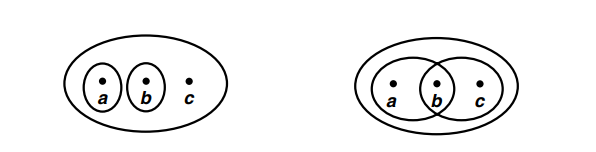
\includegraphics{figure 02.png}
\caption{\label{fig:fig2}\(~\)}
\end{figure}

\begin{example}
\protect\hypertarget{exm:unnamed-chunk-4}{}\label{exm:unnamed-chunk-4}If \(X\) is any set, the collection of all subsets of \(X\) (Power set) is a topology on \(X\). This trivail statified T1 T2 and T3 conditions. Furthur,This is called the \emph{discrete topology}.
\end{example}

\begin{example}
\protect\hypertarget{exm:unnamed-chunk-5}{}\label{exm:unnamed-chunk-5}The collection consisting of \(X\) and \(\emptyset\) only is also a topologyon \(X\). we shall call it the \emph{indiscrete topology}, or the trivial topology.
\end{example}

\begin{example}
\protect\hypertarget{exm:unnamed-chunk-6}{}\label{exm:unnamed-chunk-6}Let \(X\) be a set and let \(\tau_f\) be the collection of all subsets U of X such that \(X\setminus U\) either is finite or is all of \(X\). In oter words,
\[\tau_f:=\left\{U\subseteq X : \text{Either is finite or is all of } X\right\}\]
Let's check is \(\tau_f\) a topology. First obseve that both \(X\) and \(\emptyset\) are in \(\tau_f\) , because \(X\setminus X\) is finite and \$X\setminus \emptyset \$ is all of \(X\).So \(\tau_f\) statified the T1 condition. Now let's check the T2 condition. Let \(\{U_{\alpha}:\alpha\in I, I \text{is index set}\}\).Now we need to show that \(\cup{\alpha\in I} U_\alpha\in \tau_f\). So consider,
\[X\setminus \cup_{\alpha\in I} U_\alpha =\cap_{\alpha\in I} (X\setminus  U_\alpha).\]
Now obsevere that \cap\emph{\{\alpha\in I\} (X\setminus  U}\alpha) is finite, because each set \((X\setminus U_\alpha)\) is finite and arbitary intersection of finite sets is finite. So, \(\tau_f\) stattified the T2 condition also.
Finaly check the last condition, T3 condition. Let \(U_1,...,U_n\) are nonempty elements of \(\tau_f\) , to show that \(\Cup_i U_i \in \tau_f\) , we compute
\[X\setminus \cap_{i=1}^n U_i = \cup_{i=1}^n(X \setminus U_i).\]
Note that the set \(\cup_{i=1}^n(X \setminus U_i)\) is a finite union of finite sets and, therefore, finite. So it statisfiy the T3 condition also. Thefore \(\tau_f\) is a topology. Furthur \(\tau_f\) is called the finite \emph{complement topology}.
\end{example}

\begin{example}
\protect\hypertarget{exm:unnamed-chunk-7}{}\label{exm:unnamed-chunk-7}Let \(X\) be a set. Define \(\mathcal{T}\) to be the collection of all subsets \(U\) of \(X\) such that \(X\setminus U\) either is finite or is all of \(X\). Then \(\mathcal{T}\) defines a topology on \(X\), called finite complement topology of \(X\).
\end{example}

\hypertarget{basis-of-a-topology}{%
\section{Basis of a Topology}\label{basis-of-a-topology}}

Once we define a structure on a set, often we try to understand what the minimum data you need to specify the structure. In many cases, this minimum data is called a basis and we say that the basis generate the structure. The notion of a basis of the structure will help us to describe examples more systematically.

\begin{definition}
\protect\hypertarget{def:unnamed-chunk-8}{}\label{def:unnamed-chunk-8}Let \(X\) be a set. A basis of a topology on \(X\) is a collection \(\mathcal{B}\) of subsets in \(X\) such that

(B1) For every \(x \in X\), there exist an element \(B\) in \(\mathcal{B}\) such that \(x \in B\).

(B2) If \(x \in B_{1} \cap B_{2}\) where \(B_{1}, B_{2}\) are in \(\mathcal{B}\), then there is \(B_{3}\) in \(\mathcal{B}\) such that \(x \in B_{3} \subseteq B_{1} \cap B_{2}\).
\end{definition}

\begin{lemma}[Generating of a topology]
\protect\hypertarget{lem:unnamed-chunk-9}{}\label{lem:unnamed-chunk-9}Let \(\mathcal{B}\) be a basis of a topology on X. Define \(\mathcal{T}_{\mathcal{B}}\) to be the collection of subsets \(U \subset X\) satisfting

(G1) For every \(x \in U\), there is \(B \in \mathcal{B}\) such that \(x \in B \subset U\).

Then \(\tau_{\mathcal{B}}\) defines a topology on \(X\). Here we assume that \(\varnothing\) trivially satisfies the condition, so that \(\varnothing \in \tau_{\mathcal{B}}\).
\end{lemma}

\begin{proof}
We need to check the three axioms:
\end{proof}

\hypertarget{chapter-2-name}{%
\chapter{Chapter 2 name}\label{chapter-2-name}}

\hypertarget{chapter-03-name}{%
\chapter{Chapter 03 name}\label{chapter-03-name}}

Up to there is none.

  \bibliography{book.bib,packages.bib}

\end{document}
